%%%%%%%%%%%%%%%%%%%%%%%%%%%%%%%%%%%%%%%%%
% Cies Resume/CV
% LaTeX Template
% Version 1.1 (20/7/14)
%
% This template has been downloaded from:
% http://www.LaTeXTemplates.com
%
% Original author:
% Cies Breijs (cies@kde.nl)
% https://github.com/cies/resume with extensive modifications by:
% Vel (vel@latextemplates.com)
%
% License:
% CC BY-NC-SA 3.0 (http://creativecommons.org/licenses/by-nc-sa/3.0/)
%
%%%%%%%%%%%%%%%%%%%%%%%%%%%%%%%%%%%%%%%%%

%----------------------------------------------------------------------------------------
%	PACKAGES AND OTHER DOCUMENT CONFIGURATIONS
%----------------------------------------------------------------------------------------

\documentclass[10pt,a4paper]{article} % Font size (10-12pt) and paper size (a4paper, letterpaper, legalpaper, etc)
% Copyright (c) 2012 Cies Breijs
%
% The MIT License
%
% Permission is hereby granted, free of charge, to any person obtaining a copy
% of this software and associated documentation files (the "Software"), to deal
% in the Software without restriction, including without limitation the rights
% to use, copy, modify, merge, publish, distribute, sublicense, and/or sell
% copies of the Software, and to permit persons to whom the Software is
% furnished to do so, subject to the following conditions:
%
% The above copyright notice and this permission notice shall be included in
% all copies or substantial portions of the Software.
%
% THE SOFTWARE IS PROVIDED "AS IS", WITHOUT WARRANTY OF ANY KIND, EXPRESS OR
% IMPLIED, INCLUDING BUT NOT LIMITED TO THE WARRANTIES OF MERCHANTABILITY,
% FITNESS FOR A PARTICULAR PURPOSE AND NONINFRINGEMENT. IN NO EVENT SHALL THE
% AUTHORS OR COPYRIGHT HOLDERS BE LIABLE FOR ANY CLAIM, DAMAGES OR OTHER
% LIABILITY, WHETHER IN AN ACTION OF CONTRACT, TORT OR OTHERWISE, ARISING FROM,
% OUT OF OR IN CONNECTION WITH THE SOFTWARE OR THE USE OR OTHER DEALINGS IN THE
% SOFTWARE.

%%% LOAD AND SETUP PACKAGES

\usepackage[margin=0.75in]{geometry} % Adjusts the margins

\usepackage{multicol} % Required for multiple columns of text

\usepackage{mdwlist} % Required to fine tune lists with a inline headings and indented content

\usepackage{relsize} % Required for the \textscale command for custom small caps text

\usepackage{hyperref} % Required for customizing links
\usepackage{xcolor} % Required for specifying custom colors
\definecolor{dark-blue}{rgb}{0.15,0.15,0.4} % Defines the dark blue color used for links
\hypersetup{colorlinks,linkcolor={black},citecolor={black},urlcolor={black}} % Assigns the dark blue color to all links in the template

\usepackage{tgpagella} % Use the TeX Gyre Pagella font throughout the document
\usepackage[T1]{fontenc}
\usepackage{microtype} % Slightly tweaks character and word spacings for better typography

\usepackage{graphicx}

% some commands to add a timestamp
\usepackage{datetime}

\usepackage{eso-pic}

\usepackage{amsmath}

\settimeformat{hhmmsstime}
\AddToShipoutPicture{%
     \AtTextLowerLeft{%
         \put(0, -45){\ifdefined\shortcv{\normalsize \it \color{gray} Download full CV \href{https://raw.githubusercontent.com/sebastian-lapuschkin-sideprojects/latex-cv/master/cv.pdf}{[here]}.}\else{}\fi}
         \put(273,-45){\normalsize \it \color{gray} Last updated on \today\ -- \currenttime}%
     }%
}


\pagestyle{empty} % Stop page numbering

%----------------------------------------------------------------------------------------
%	DEFINE STRUCTURAL COMMANDS
%----------------------------------------------------------------------------------------

\newenvironment{indentsection} % Defines the indentsection environment which indents text in sections titles
{\begin{list}{}{\setlength{\leftmargin}{\newparindent}\setlength{\parsep}{0pt}\setlength{\parskip}{0pt}\setlength{\itemsep}{0pt}\setlength{\topsep}{0pt}}}{\end{list}}

\newenvironment{unindentsection} % Defines the uindentsection environment which indents text in sections titles
{\begin{list}{}{\setlength{\leftmargin}{0pt}\setlength{\parsep}{0pt}\setlength{\parskip}{0pt}\setlength{\itemsep}{0pt}\setlength{\topsep}{0pt}}}{\end{list}}


\newcommand*\maintitle[2]{\noindent{\LARGE \textbf{#1}}\ \ \ \emph{#2}\vspace{0.3em}} % Main title (name) with date of birth or subtitle

\newcommand*\roottitle[1]{\subsection*{#1}\vspace{-0.3em}\nopagebreak[4]} % Top level sections in the template

\newcommand{\headedsection}[3]{
\nopagebreak[4]
\begin{unindentsection}
\item[]
\textscale{1.1}
{#1}
\hfill#2#3
\end{unindentsection}
\nopagebreak[4]
} % Section title used for a new employer

\newcommand{\headedsubsection}[3]{\nopagebreak[4]\begin{indentsection}\item[]\textbf{#1}\hfill\emph{#2}#3\end{indentsection}\nopagebreak[4]} % Section title used for a new position

\newcommand{\bodytext}[1]{
\nopagebreak[4]
\begin{unindentsection}
\item[]
#1
\end{unindentsection}
\pagebreak[2]} % Body text (indented)

\newcommand{\inlineheadsection}[2]{\begin{basedescript}{\setlength{\leftmargin}{\doubleparindent}}\item[\hspace{\newparindent}\textbf{#1}]#2\end{basedescript}\vspace{-1.7em}} % Section title where body text starts immediately after the title

\newcommand*\acr[1]{\textscale{.85}{#1}} % Custom acronyms command

\newcommand*\bull{\ \ \raisebox{-0.365em}[-1em][-1em]{\textscale{4}{$\cdot$}} \ } % Custom bullet point for separating content

\newlength{\newparindent} % It seems not to work when simply using \parindent...
\addtolength{\newparindent}{\parindent}

\newlength{\doubleparindent} % A double \parindent...
\addtolength{\doubleparindent}{\parindent}

\newcommand{\breakvspace}[1]{\pagebreak[2]\vspace{#1}\pagebreak[2]} % A custom vspace command with custom before and after spacing lengths
\newcommand{\nobreakvspace}[1]{\nopagebreak[4]\vspace{#1}\nopagebreak[4]} % A custom vspace command with custom before and after spacing lengths that do not break the page

\newcommand{\spacedhrule}[2]{\breakvspace{#1}\hrule\nobreakvspace{#2}} % Defines a horizontal line with some vertical space before and after it

%----------------------------------------------------------------------------------------
%	DEFINE ADDITIONAL COMMANDS
%----------------------------------------------------------------------------------------

\newcommand{\todo}[1]{{\color{red}{#1}}}
\newcommand{\vstep}{\vspace{3pt}}
 % Include structure.tex which contains packages and document layout definitions

\hyphenation{Some-long-word} % Specify custom hyphenation points in words with dashes where you would like hyphenation to occur, or alternatively, don't put any dashes in a word to stop hyphenation altogether

\begin{document}

%----------------------------------------------------------------------------------------
%	NAME AND CONTACT INFORMATION
%----------------------------------------------------------------------------------------

%TODO: Extend summay text to push EDUCATION to page 2.
%TODO generally improve texts
\noindent
\begin{minipage}{.8\textwidth}

\maintitle{Dr. Sebastian Lapuschkin}{(n\'e Bach), December 16, 1986}  % Your name and date of birth or subtitle

\noindent\href{mailto:sebastian@lapuschkin.com}{sebastian@lapuschkin.com}\bull % Your email address
\textsmaller{+}49 (177) 483-2754\bull % Your phone number(s)
\href{https://scholar.google.com/citations?user=wpLQuroAAAAJ}{Google Scholar}
\\
\href{https://github.com/sebastian-lapuschkin}{github.com/sebastian-lapuschkin}\bull % github
\href{https://www.linkedin.com/in/sebastian-lapuschkin}{linkedin.com/in/sebastian-lapuschkin} % linkedin
\\
%\href{https://orcid.org/0000-0002-0762-7258}{https://orcid.org/0000-0002-0762-7258}% orcid
%\bull
%\href{https://scholar.google.com/citations?user=wpLQuroAAAAJ}{https://scholar.google.com/citations?user=wpLQuroAAAAJ}% google scholar
%\\
Kaiserin-Augusta-Allee 92\bull 10589 Berlin \bull Berlin\bull Germany % Your address
\end{minipage}
\begin{minipage}{.2\textwidth}
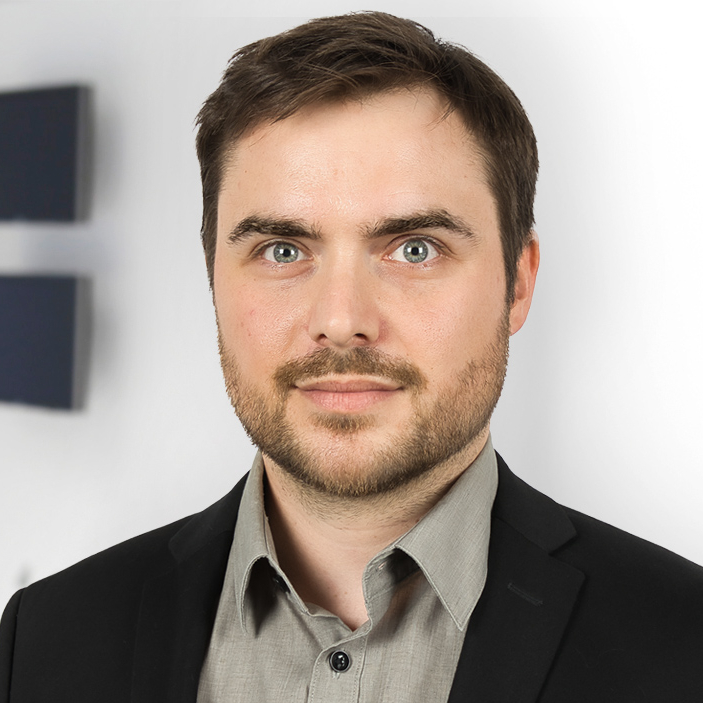
\includegraphics[width=\textwidth]{resources/mug-2021.jpg}
\end{minipage}


\spacedhrule{0.9em}{-0.4em} % Horizontal rule - the first bracket is whitespace before and the second is after

%----------------------------------------------------------------------------------------
%	SUMMARY SECTION
%----------------------------------------------------------------------------------------

\roottitle{Short Bio} % Root section title

\vspace{-1.3em} % Reduce whitespace after the Summary heading and the two-column content

\begin{multicols}{2}  % Start a two-column layout
\noindent

Sebastian Lapuschkin received the Ph.D. degree with distinction from the Berlin Institute of Technology in 2018
for his pioneering contributions to the field of Explainable Artificial Intelligence (XAI) and interpretable machine learning.
From 2007 to 2013 he studied computer science (B. Sc. and M. Sc.) at the Berlin Institute of Technology,
with a focus on software engineering and machine learning.

Currently, he is the Head of the Explainable Artificial Intelligence at Fraunhofer Heinrich Hertz Institute (HHI) in Berlin.
He is recipient of multiple awards, including the Hugo-Geiger-Prize for outstanding doctoral achievement and the 2020 Pattern Recognition Best Paper Award.
His current work is focused on actionable Explainable AI for the interpretation, holistic analysis and rectification of machine learning system behavior.
Further research interests include efficient machine learning and data analysis, data and algorithm visualization.

Sebastian loves automation and woodland hiking (not simultaneously).

%Besides his professional endeavours, Sebastian enjoys automating repeating office work
\end{multicols}

\spacedhrule{0.5em}{-0.4em} % Horizontal rule - the first bracket is whitespace before and the second is after



%----------------------------------------------------------------------------------------
%	EXPERIENCE SECTION
%----------------------------------------------------------------------------------------

\roottitle{Professional Experience} % Top level section

\headedsection % Employer name which can include a hyperlink and location/URL on the right side of the page
{\href{https://www.hhi.fraunhofer.de/}{Fraunhofer Heinrich Hertz Institute}/\href{https://www.hhi.fraunhofer.de/}{\acr{HHI}}}
{\textsc{Berlin, Germany}}
{
    \headedsubsection
    {Head of Explainable Artificial Intelligence}
    {Jan '21 -- present}
    {
        \bodytext{
            Group Leadership and direction of XAI research.

            \emph{Research:}
            Work towards the next generation of Explainable AI approaches
            and XAI-based model improvement by, e.g.,
            \href{https://scholar.google.com/citations?view_op=view_citation&citation_for_view=wpLQuroAAAAJ:Wp0gIr-vW9MC}{increasing efficiency}
            (\href{https://scholar.google.com/citations?view_op=view_citation&citation_for_view=wpLQuroAAAAJ:TFP_iSt0sucC}{see also})
            and
            \href{https://scholar.google.com/citations?view_op=view_citation&citation_for_view=wpLQuroAAAAJ:iH-uZ7U-co4C}{debugging model training, reasoning and datasets}.
            Provision of powerful modified backprop XAI for Pytorch models,
            and tools for reproducible XAI evaluations to the community via
            \href{https://github.com/chr5tphr/zennit}{Zennit}
            and
            \href{https://github.com/understandable-machine-intelligence-lab/Quantus}{Quantus}.

            \vstep

            \emph{Further responsibilities:}
            Project management and (funding) acquisition.
            Recruitment and guidance of research staff.

        }
    }

    \headedsubsection % Job title entry for the current employer
    {Tenured Researcher}
    {Jan '19 -- present}
    {
        \bodytext{
            PostDoc research position in the Machine Learning Group at Fraunhofer HHI.

            \emph{Research:}
            Development of \href{https://scholar.google.com/citations?view_op=view_citation&citation_for_view=wpLQuroAAAAJ:5nxA0vEk-isC}{Spectral Relevance Analysis},
            automating the detection of ``Clever Hans'' moments in machine learning.
            \href{https://scholar.google.com/citations?view_op=view_citation&citation_for_view=wpLQuroAAAAJ:3fE2CSJIrl8C}{Measurably increasing}
            the
            \href{https://scholar.google.com/citations?view_op=view_citation&citation_for_view=wpLQuroAAAAJ:MXK_kJrjxJIC}{explanation quality} of
            local XAI.
            Provision of modified backprop XAI in Keras/Tensorflow via
            \href{https://github.com/albermax/innvestigate}{iNNvestigate}.

            \vstep
            \emph{Further responsibilities:}
            Project (funding) acquisition.
            Recruitment and guidance of PhD students and student research assistants.
        }
    }

    \headedsubsection % Job title entry for the current employer
    {Research Associate}
    {Oct '14 -- Dec '18}
    {
        \bodytext{
            Founding member of the Machine Learning Group at Fraunhofer HHI.

            \emph{Research:}
            Furthering XAI research with the
            \href{https://scholar.google.com/citations?view_op=view_citation&hl=de&user=wpLQuroAAAAJ&citation_for_view=wpLQuroAAAAJ:u-x6o8ySG0sC}{development} and
            \href{https://scholar.google.com/citations?view_op=view_citation&hl=de&user=wpLQuroAAAAJ&citation_for_view=wpLQuroAAAAJ:u5HHmVD_uO8C}{evaluation} of corresponding methods,
            as well as applications in
            \href{https://scholar.google.com/citations?view_op=view_citation&hl=de&user=wpLQuroAAAAJ&citation_for_view=wpLQuroAAAAJ:9yKSN-GCB0IC}{various expert domains},
            resulting in
            \href{https://scholar.google.com/citations?user=wpLQuroAAAAJ}{several highly cited publications},
            open source
            \href{https://scholar.google.com/citations?view_op=view_citation&hl=de&user=wpLQuroAAAAJ&citation_for_view=wpLQuroAAAAJ:2osOgNQ5qMEC}{software}
            tools and
            \href{https://github.com/sebastian-lapuschkin/lrp_toolbox}{repositories},
            and the \href{https://scholar.google.com/citations?view_op=view_citation&hl=de&user=wpLQuroAAAAJ&citation_for_view=wpLQuroAAAAJ:d1gkVwhDpl0C}{first recorded encounter} of the
            \href{https://scholar.google.com/citations?view_op=view_citation&citation_for_view=wpLQuroAAAAJ:5nxA0vEk-isC}{``Clever Hans'' effect}
            in machine learning via XAI.

            \vstep

            \emph{Other contributions:}
            Minor contributions to the h.266 (VVC) video codec via learnable intra-frame prediction filters.
            Planning and conceptualization of an HPC cluster with modern GPU hardware implemented at Fraunhofer HHI.
            Development and showcasing
            \href{https://lrpserver.hhi.fraunhofer.de/}{multiple XAI demos}
            in international events.

            \vstep

            Additional supervision by
            \href{https://scholar.google.com/citations?user=7aQwO08AAAAJ}{Prof. Dr. Wojciech Samek}.

        }
    }
}

%------------------------------------------------

\headedsection % Employer name which can include a hyperlink and location/URL on the right side of the page
{\href{http://www.tu-berlin.de/ }{Berlin Institute of Technology}/\href{http://www.tu-berlin.de/ }{\acr{TU Berlin}}}
{\textsc{Berlin, Germany}}
{
    \headedsubsection % Job title entry for the current employer
    {Research Associate}
    {Sep '13 -- Sep '14}
    {
        \bodytext{
            \emph{Research:}
            Formalization and development of the ``\href{https://scholar.google.com/citations?view_op=view_citation&hl=de&user=wpLQuroAAAAJ&citation_for_view=wpLQuroAAAAJ:YsMSGLbcyi4C}{Layer-wise Relevance Propagation}'' (LRP) method
            of Explainable AI
            for explaining individual predictions of nonlinear machine learning models.

            Supervision by
            \href{https://scholar.google.com/citations?user=jplQac8AAAAJ}{Prof. Dr. Klaus-Robert M\"uller} and
            \href{https://scholar.google.com/citations?user=5B8CTlEAAAAJ}{Prof. Dr. Alexander Binder}.

        }
    }

    \headedsubsection % Job title entry for the current employer
    {Student Research- \& Teaching Assistant}
    {Oct '11 -- Aug '13}
    {
        \bodytext{


            \emph{Research:}
            Structure and cell type detection in large histopathology images using Bag of Words features and SVM classifiers.
            Development of XAI for the pipeline.

            Research assistant to
            \href{https://scholar.google.com/citations?user=5B8CTlEAAAAJ}{Prof. Dr. Alexander Binder}
            at the department for machine learning at TU Berlin.

            \vstep


            \emph{Teaching:}
            Preparation and lecturing of exercise sessions complementing the lectures
            ``Machine Learning~1'' and ``Machine Learning~2 -- Theory and Application''.
            Visualization and animation of data and learning algorithms discussed in the lecture.

            Teaching assistant to
            \href{https://scholar.google.com/citations?user=jplQac8AAAAJ}{Prof. Dr. Klaus-Robert M\"uller} and
            \href{https://scholar.google.com/citations?user=VYi_04kAAAAJ}{Prof. Dr. Dr. Franz Kir\'aly}.
        }
    }

    \headedsubsection % Job title entry for the current employer
    {Student Teaching Assistant}
    {Oct '09 -- Sep '11}
    {
        \bodytext{

            Course instruction for algorithmic and practical foundations of computer science (B.Sc.):
            Basic and advanced Java development, software engineering and OOP concepts, algorithms on image and graph data, among others.

            Teaching assistant to
            \href{https://scholar.google.com/citations?user=KNwXLLsAAAAJ}{Prof. Dr. Marc Alexa},
            \href{https://scholar.google.com/citations?user=mvOSfFAAAAAJ}{Prof. Dr. Odej Kao} and
            \href{https://scholar.google.com/citations?user=83OxU_4AAAAJ}{Prof. Dr. Oliver Brock}.

        }
    }
}

%------------------------------------------------

%\begin{center}
%\textit{Please refer to \href{https://www.linkedin.com/in/sebastian-lapuschkin-903b3b140/}{my Linkedin profile} for the complete list of work experiences along with recommendations.}
%\end{center}

%------------------------------------------------

\spacedhrule{0.5em}{-0.4em} % Horizontal rule - the first bracket is whitespace before and the second is after



%----------------------------------------------------------------------------------------
%	EDUCATION SECTION
%----------------------------------------------------------------------------------------

\roottitle{Education} % Top level section

\headedsection % Employer name which can include a hyperlink and location/URL on the right side of the page
{\href{http://www.tu-berlin.de/ }{Berlin Institute of Technology}/\href{http://www.tu-berlin.de/ }{\acr{TU Berlin}}}
{\textsc{Berlin, Germany}}
{
    \headedsubsection % Job title entry for the current employer
    {PhD in Machine Learning \textnormal{(with distinction / ``summa cum laude'')}}
    {2013 -- 2018}
    {
        \bodytext{
            Research and application of methods of \emph{Explainable AI (XAI)}:

            \href{https://scholar.google.com/citations?view_op=view_citation&citation_for_view=wpLQuroAAAAJ:YsMSGLbcyi4C}{Layer-wise Relevance Propagation},
            \href{https://scholar.google.com/citations?view_op=view_citation&citation_for_view=wpLQuroAAAAJ:u-x6o8ySG0sC}{Deep Taylor Decomposition},
            \href{https://scholar.google.com/citations?view_op=view_citation&citation_for_view=wpLQuroAAAAJ:5nxA0vEk-isC}{Spectral Relevance Analysis}, \dots

            \href{http://dx.doi.org/10.14279/depositonce-7942}{Thesis: ``Opening the machine learning black box with Layer-wise Relevance Propagation''}

            Supervision headed by \href{https://scholar.google.com/citations?user=jplQac8AAAAJ}{Prof. Dr. Klaus-Robert M\"uller}.
            }
    }

    \headedsubsection % Job title entry for the current employer
    {Master of Science in Computer Science % \textnormal{(1.4 / ``very good'' / GPA 3.7)}
    }
    {2010 -- 2013}
    {
        \bodytext{
            Focus on machine learning, computer vision and large scale data analysis.

            \href{https://drive.google.com/file/d/106Wjpnc-Qm8FVEAppVDekpYHRT43Emrf/view?usp=sharing}{Thesis: ``On Pixel-wise Predictions from Image-wise Bag of Words Classification''} % (Grade: 1.0 /  A)

            Supervision headed by \href{https://scholar.google.com/citations?user=5B8CTlEAAAAJ}{Prof. Dr. Alexander Binder}.
        }
    }

    \headedsubsection % Job title entry for the current employer
    {Bachelor of Science in Computer Science % \textnormal{(2.0 / ``good'' / GPA 3.0)}
    }
    {2007 -- 2010}
    {
        \bodytext{
            Focus on Algorithms and Software Development

            \href{https://drive.google.com/file/d/1bn-PPMmC4ejwy-Fu42Pzqcu_M6IgHjBH/view?usp=sharing}{Thesis: ``Keyword-Based Image Browsing of Large Image Databases''} % (Grade: 1.0 / A)

            Supervision headed by \href{https://scholar.google.com/citations?user=qhEK194AAAAJ}{Prof. Dr. Kristian Hildebrand}.

            }
    }
}

%------------------------------------------------

\headedsection % Employer name which can include a hyperlink and location/URL on the right side of the page
{\href{https://www.deutschhaus.de/ }{Deutschhaus-Gymnasium}/\href{https://www.deutschhaus.de/ }{\acr{DHG}}}
{\textsc{W\"urzburg, Germany}}
{
\headedsubsection % Job title entry for the current employer
{Abitur \textnormal{(pre-university secondary education)}}
{1998 -- 2007}
 {}
}

\spacedhrule{0.5em}{-0.4em} % Horizontal rule - the first bracket is whitespace before and the second is after
%----------------------------------------------------------------------------------------
%	PROJECTS SECTION
%----------------------------------------------------------------------------------------

\roottitle{Research Projects}
\inlineheadsection{DAKI-FWS (2021-12 -- 2024-11)}{\href{https://www.hhi.fraunhofer.de/en/departments/ai/projects/daki-fws.html}{Data- and AI-supported Early Warning System}}
\inlineheadsection{iToBoS (2021-04 -- 2025-03)}{\href{https://www.hhi.fraunhofer.de/en/departments/ai/projects/itobos.html}{Intelligent Total Body Scanner}}
\inlineheadsection{BerDiBa (2021-01 -- 2023-12)}{\href{https://www.hhi.fraunhofer.de/en/departments/ai/projects/berdiba.html}{Berlin Digital Rail Operations}}
\inlineheadsection{TraMeExCo (2018-09 -- 2021-08)}{\href{https://www.hhi.fraunhofer.de/en/departments/ai/projects/trameexco.html}{Transparent Medical Expert Companion}}

\spacedhrule{1.6em}{-0.4em} % Horizontal rule - the first bracket is whitespace before and the second is after
%----------------------------------------------------------------------------------------
%	SKILLS SECTION
%----------------------------------------------------------------------------------------

\roottitle{Skills} % Top level section
\inlineheadsection
{Technical:}
{
    %\bodytext{
    Various Software Languages, packages and environments, e.g.,\\
    Python (NumPy, PyTorch, \dots), Matlab, Linux, bash, git, subversion, Slurm, Sun Grid Engine, \dots
    %Matlab, HTML, C\#, C++, C, Java, lua, SQL, \dots )
    %}
}

\vspace{5pt}
\inlineheadsection
{Scientific working and writing:}
{
    %\bodytext{
        LaTeX, Inkscape, WYSIWYG word processors, \dots
        %}
}

\vspace{5pt}
\inlineheadsection
{Machine Learning:}
{
    %\bodytext{
        Development, application and evaluation of, e.g.,\\
        SVMs, DNNs, processing pipelines, embeddings, clusterings, \dots
    %}
}

\vspace{5pt}
\inlineheadsection{Domain Knowledge:}
{
   %\bodytext{
       text, audio, video, images, time series, biomechanical and biomedical data, \dots
   %}
}


%------------------------------------------------

\vspace{5pt}
\inlineheadsection % Special section that has an inline header with a 'hanging' paragraph
{Natural languages:}
{
    %\bodytext{
    German \textit{(native)}, English \textit{(full professional proficiency)}
    %}
}

%------------------------------------------------

\spacedhrule{1.6em}{-0.4em} % Horizontal rule - the first bracket is whitespace before and the second is after

% %----------------------------------------------------------------------------------------
% %	INTERESTS SECTION
% %----------------------------------------------------------------------------------------

% \roottitle{Interests} % Top level section

% \inlineheadsection % Special section that has an inline header with a 'hanging' paragraph
% {In no particular order:}
% {
%     Data visualization,
%     programming,
%     working out,
%     (couch-coop) video games,
%     (audio) books,
%     over-engineered automation of daily tasks,
%     the outdoors and spending time with the wife, dogs \& kid hiking in the woods,
%     vegan food (cooking and eating, much).
% }

% %----------------------------------------------------------------------------------------

% \spacedhrule{1.6em}{-0.4em} % Horizontal rule - the first bracket is whitespace before and the second is after


%----------------------------------------------------------------------------------------
%	AWARDS SECTION
%----------------------------------------------------------------------------------------

\roottitle{Awards} % Top level section

\inlineheadsection
{Pattern Recognition Best Paper Award and Pattern Recognition Medal (2020)}
{
    for the paper\\
    \href{https://doi.org/10.1016/j.patcog.2016.11.008}{\qquad ``Explaining NonLinear Classification Decisions with Deep Taylor Decomposition''}
}

\vspace{5pt}
\inlineheadsection % Special section that has an inline header with a 'hanging' paragraph
{Hugo-Geiger-Prize (2019, 1st place)}
{
    F\"orderpreis f\"ur herausragende Promotionsleistungen
}

\vspace{5pt}
\inlineheadsection % Special section that has an inline header with a 'hanging' paragraph
{Freunde des HHI (2019)}
{
    F\"orderpreis f\"ur exzellente wissenschaftliche Arbeiten am HHI
}

\vspace{5pt}
\inlineheadsection % Special section that has an inline header with a 'hanging' paragraph
{ERCIM (2019, finalist)}
{
    Cor Baayen Young Researcher Award
}

\vspace{5pt}
\inlineheadsection % Special section that has an inline header with a 'hanging' paragraph
{Best Paper Prize (2016)}
{
    ICML'16 Workshop on Visualization for Deep Learning
}

%----------------------------------------------------------------------------------------

\spacedhrule{1.6em}{-0.4em} % Horizontal rule - the first bracket is whitespace before and the second is after
%----------------------------------------------------------------------------------------
%	Patents Section
%----------------------------------------------------------------------------------------

\roottitle{Patents} % Top level section
%params: 1:countrycode, 2:patentid, 3:title, 4:link, 5:granteddate
\newcommand{\patentref}[5]{\href{#4}{#1 #2} ``#3'' (granted #5)}
%params: 1:countrycode, 2:patenpublicationtid, 3:title, 4:link, 5:pubdate
\newcommand{\patentpubref}[5]{\href{#4}{#1 #2} ``#3'' (published #5)}
\headedsection{\bf Pruning and/or Quantizing Machine Learning Predictors }
{
    \begin{enumerate}
        \item [] \patentpubref{EP}
                                {3991102 A1}
                                {Pruning and/or Quantizing Machine Learning Predictors}
                                {https://patents.google.com/patent/EP3991102A1/en}
                                {2022-05-04}
        \item [] \patentpubref{US}
                                {2022/0114455 A1}
                                {Pruning and/or Quantizing Machine Learning Predictors}
                                {https://patentimages.storage.googleapis.com/36/80/74/01e3b22ef42a94/US20220114455A1.pdf}
                                {2022-04-14}
        \item [] \patentpubref{WO}
                                {2020/260656 A1}
                                {Pruning and/or Quantizing Machine Learning Predictors}
                                {https://patentimages.storage.googleapis.com/27/0b/d4/e3edd382b114fe/WO2020260656A1.pdf}
                                {2020-12-30}
    \end{enumerate}
}

\headedsection % Special section that has an inline header with a 'hanging' paragraph
{\bf Relevance Score Assignment for Artificial Neural Networks}
{
    \begin{enumerate}
        \item[] \patentref{CN}
                          {107636693}
                          {Relevance Score Assignment for Artificial Neural Networks}
                          {https://patentimages.storage.googleapis.com/f0/97/e9/24faaaca17252c/CN107636693B.pdf}
                          {2022-01-11}

        \item [] \patentref{EP}
                           {3271863}
                           {Relevance Score Assignment for Artificial Neural Network}
                           {https://patentimages.storage.googleapis.com/0c/a1/63/580ce6ff29f011/EP3271863B1.pdf}
                           {2021-07-28}

        \item [] \patentref{JP}
                           {6725547}
                           {Relevance Score Assignment for Artificial Neural Networks}
                           {https://patentimages.storage.googleapis.com/91/ba/cc/36792436528537/JP6725547B2.pdf}
                           {2020-07-22}

        \item [] \patentref{KR}
                           {102130162}
                           {Assignment of Relevance Scores for Artificial Neural Networks}
                           {https://patentimages.storage.googleapis.com/80/b5/17/210f687345bb31/KR102130162B1.pdf}
                           {2020-07-06}

        \item [] \patentref{CA}
                           {2979579}
                           {Relevance Score Assignment for Artificial Neural Networks}
                           {https://patents.google.com/patent/CA2979579A1/en}
                           {2020-02-18}

        \item [] \patentref{RU}
                           {2703343}
                           {Relevancy Assessment for Artificial Neural Networks}
                           {https://patentimages.storage.googleapis.com/8d/ce/b5/70ef43a6d0f6e5/RU2703343C2.pdf}
                           {2019-10-16}
    \end{enumerate}
}

%----------------------------------------------------------------------------------------


%----------------------------------------------------------------------------------------
\spacedhrule{0.5em}{-0.4em} % Horizontal rule - the first bracket is whitespace before and the second is after
%----------------------------------------------------------------------------------------
%	Orals SECTION
%----------------------------------------------------------------------------------------
\roottitle{Talks \& Lectures} % Top level section
%params: 1:authors, 2:date, 3:title, 4:locationorevent
\newcommand{\talkref}[4]{``#3'' (#2).\\\textit{#4}}
%params: 1:authors, 2:date, 3:title, 4:locationorevent, 5:note
\newcommand{\talkrefwnote}[5]{``#3'' (#2).\\\textit{#4, (#5)}}

\headedsection
{Talks}{excludes internal/confidential events}
{
\begin{enumerate}
    \item \talkrefwnote{\textbf{Sebastian Lapuschkin}}
                    {2021-06-03}
                    {Beyond Explaining}
                    {Melanoma Patient Network Europe Meet-up -- MPNE meets AI }
                    {invited talk}
    \item \talkrefwnote{\textbf{Sebastian Lapuschkin}}
                    {2021-05-05}
                    {Beyond Explaining: Explainable AI for Model Improvement}
                    {Sensor and Measurement Science International 2021}
                    {invited talk}
    \item \talkref{\textbf{Sebastian Lapuschkin}}
                    {2020-11-12}
                    {Efficient and Effective Neural Network Pruning with Layer-wise Relevance Propagation}
                    {Machine Learning Seminar at Fraunhofer HHI / Technische Universität Berlin}
    \item \talkref{\textbf{Sebastian Lapuschkin}}
                    {2020-07-21}
                    {Towards Best Practice in Explaining Neural Network Decisions with LRP}
                    {IEEE World Congress on Computational Intelligence 2020 / IJCNN 2020}
    \item \talkrefwnote{\textbf{Sebastian Lapuschkin}}
                    {2020-07-18}
                    {XAI for Analyzing and Unlearning Spurious Correlations in ImageNet}
                    {XXAI: Extending Explainable AI Beyond Deep Models and Classifiers}
                    {ICML 2020 Workshop}
    \item \talkrefwnote{\textbf{Sebastian Lapuschkin}}
                    {2020-07-02}
                    {XAI via LRP and SpRAy}
                    {Ada Day at Ada Lovelace Center / Fraunhofer IIS}
                    {invited talk}
    \item \talkref{\textbf{Sebastian Lapuschkin}}
                    {2020-02-18}
                    {Interpretable Machine Learning through Layer-wise Relevance Propagation}
                    {Fraunhofer Symposium Netzwert 2020}
    \item \talkref{\textbf{Sebastian Lapuschkin}}
                    {2019-12-12}
                    {Interpretable Machine Learning through Layer-wise Relevance Propagation}
                    {Gesellschaft von Freunden des HHI e.V.}
    \item \talkrefwnote{\textbf{Sebastian Lapuschkin}}
                    {2019-09-26}
                    {Explainable Artificial Intelligence --- Opening the Machine Learning Black Box with Layer-wise Relevance Propagation}
                    {AMA Wissenschaftsrat 2019}
                    {invited talk}
    \item \talkrefwnote{\textbf{Sebastian Lapuschkin}}
                    {2019-07-16}
                    {Finding Clever Hans}
                    {Universität Bamberg}
                    {invited talk \& interview}
    \item \talkrefwnote{\textbf{Sebastian Lapuschkin}}
                    {2019-02-25}
                    {AI -- Opening the Black Box}
                    {Robert Koch Institut}
                    {invited talk}
    \item \talkref{\textbf{Sebastian Lapuschkin}}
                    {2019-02-22}
                    {AI -- Opening the Black Box}
                    {Technology Innovation Day -- 91 Years HHI}
    \item \talkref{\textbf{Sebastian Lapuschkin}}
                    {2017-10-27}
                    {Understanding and Comparing Deep Neural Networks for Age and Gender Classification}
                    {ICCV'17 Workshop on Analysis and Modeling of Faces and Gestures}
\end{enumerate}
}

% added to cover ugly page break right after section head
\headedsection
{Lectures}{}
{
\begin{enumerate}
    \item \talkrefwnote{\textbf{Sebastian Lapuschkin}}
                    {2022-12-13/14/16}
                    {Explainable AI}
                    {Universitat de Girona}
                    {3-day lecture series as part of the Machine Learning Seminar}
    \item \talkref{\textbf{Sebastian Lapuschkin}}
                    {2021-08-27}
                    {XAI BEYOND EXPLAINING: Using Explainability for Improving Deep Machine Learning Models}
                    {2nd Summer School on Machine Learning in Bioinformatics | Higher School or Economics Moscow}
    \item \talkref{\textbf{Sebastian Lapuschkin}}
                    {2020-08}
                    {Neuronale Netze mit LRP (richtig) erklären}
                    {KI-Campus | Die Lernplattform für Künstliche Intelligenz}
    \item \talkref{\textbf{Sebastian Lapuschkin}}
                    {2019-08-16}
                    {Explainable Artificial Intelligence --- Opening the Machine Learning Black Box with Layer-wise Relevance Propagation}
                    {SIMULA Summer School on Smart cities for a Sustainable Energy Future - From Design to Practice}
\end{enumerate}
}


%----------------------------------------------------------------------------------------
\spacedhrule{0.5em}{-0.4em} % Horizontal rule - the first bracket is whitespace before and the second is after
%----------------------------------------------------------------------------------------
%	PUBLICATIONS SECTION
%----------------------------------------------------------------------------------------

\roottitle{Publications} % Top level section
%params: 1:authors, 2:year, 3:title, 4:publishedin, 5:pages, 6:link
\newcommand{\journalref}[6]{#1 (#2).\\``#3''.\\In: \href{#6}{\textit{#4} #5}}
%params: 1:authors, 2:year, 3:title, 4:publishedin, 5:pages, 6:link, 7:note
\newcommand{\journalrefwnote}[7]{#1 (#2).\\``#3''.\\In: \href{#6}{\textit{#4} #5}. \textit{#7}}
%params: 1:authors, 2:year, 3:title, 4:publishedin, 5:pages, 6:link
\newcommand{\conferenceref}[6]{#1 (#2).\\``#3''.\\In: \href{#6}{\textit{#4} #5}}
%params: 1:authors, 2:year, 3:title, 4:publishedin, 5:pages, 6:link, 7:note
\newcommand{\conferencerefwnote}[7]{#1 (#2).\\``#3''.\\In: \href{#6}{\textit{#4} #5}. \textit{#7} }
%params: 1:authors, 2:year, 3:title, 4:publishedin, 5:pages, 6:link, 7:publisher
\newcommand{\bookchapterref}[7]{#1 (#2).\\``#3''.\\In: \href{#6}{\textit{#4} #5}. #7}
%params: 1:authors, 2:year, 3:title, 4:publishedin, 5:link
\newcommand{\preprintref}[5]{#1 (#2).\\``#3''.\\In: \href{#5}{\textit{#4}}}
%params: 1:authors, 2:year, 3:title, 4:publishedin, 5:link, 6:note
\newcommand{\preprintrefwnote}[6]{#1 (#2).\\``#3''.\\In: \href{#5}{\textit{#4}}. \textit{#6}}

\headedsection % Employer name which can include a hyperlink and location/URL on the right side of the page
{Journal Articles}{ }
{
\begin{enumerate}

    \item \journalrefwnote{Rieckmann A, Dworzynski P, Arras L, \textbf{Lapuschkin S}, Samek W, Onyebuchi A A, Rod N H, Ekstr{\o}m C T}
                        {2022}
                        {Causes of Outcome Learning: A Causal Inference-inspired Machine Learning Approach to Disentangling Common Combinations of Potential Causes of a Health Outcome}
                        {International Journal of Epidemiology}
                        {dyac078}
                        {https://doi.org/10.1093/ije/dyac078}
                        {\href{https://github.com/ekstroem/cool}{https://github.com/ekstroem/cool}}

    \item \journalref{Slijepcevic D, Horst F, \textbf{Lapuschkin S}, Horsak B, Raberger A-M, Kranzl A, Samek W, Breiteneder C, Sch\"ollhorn W I and Zeppelzauer M}
                        {2022}
                        {Explaining Machine Learning Models for Clinical Gait Analysis}
                        {ACM Transactions on Computing for Healthcare}
                        {3(2):14:1-27}
                        {https://doi.org/10.1145/3474121}


    \item \journalref{Anders C J, Weber L, Neumann D, Samek W, M\"uller K-R and \textbf{Lapuschkin S}}
                        {2022}
                        {Finding and Removing Clever Hans: Using Explanation Methods to Debug and Improve Deep Models}
                        {Information Fusion}
                        {77:261-295}
                        {https://www.sciencedirect.com/science/article/pii/S1566253521001573}


    \item \journalref{Sun J, \textbf{Lapuschkin S}, Samek W and Binder A}
                       {2022}
                       {Explain and Improve: LRP-inference Fine-tuning for Image Captioning Models}
                       {Information Fusion}
                       {77:233-246}
                       {https://www.sciencedirect.com/science/article/pii/S1566253521001494}

    \item \journalref{Samek W, Montavon G, \textbf{Lapuschkin S}, Anders C J, and M\"uller K-R}
                        {2021}
                        {Explaining Deep Neural Networks and Beyond: A Review of Methods and Applications}
                        {Proceedings of the IEEE}
                        {109(3):247-278}
                        {https://doi.org/10.1109/JPROC.2021.3060483}

    \item \journalref{Yeom S-K, Seegerer P, \textbf{Lapuschkin S}, Binder A, Wiedemann S, M\"uller K-R and Samek W}
                        {2021}
                        {Pruning by Explaining: A Novel Criterion for Deep Neural Network Pruning}
                        {Pattern Recognition}
                        {115:107899}
                        {https://doi.org/10.1016/j.patcog.2021.107899}

    \item \journalref{Aeles J, Horst F, \textbf{Lapuschkin S}, Lacourpaille L, and Hug F}
                        {2021}
                        {Revealing the Unique Features of Each Individual's Muscle Activation Signatures}
                        {Journal of the Royal Society Interface}
                        {18(174):20200770}
                        {https://doi.org/10.1098/rsif.2020.0770}

    \item \journalref{Horst F, Slijepcevic D,  Zeppelzauer M, Raberger AM, \textbf{Lapuschkin S}, Samek W,  Sch{\"o}llhorn WI, Breiteneder C, and Horsak B}
                        {2020}
                        {Explaining Automated Gender Classification of Human Gait}
                        {Gait \& Posture}
                        {81(S1):159-160}
                        {https://doi.org/10.1016/j.gaitpost.2020.07.114}

    \item \journalref{H\"agele M, Seegerer P, \textbf{Lapuschkin S}, Bockmayr M, Samek W, Klauschen F, M\"uller K-R and Binder A}
                        {2020}
                        {Resolving Challenges in Deep Learning-based Analyses of Histopathological Images using Explanation Methods}
                        {Scientific Reports}
                        {10:6423}
                        {https://doi.org/10.1038/s41598-020-62724-2}

    \item \journalrefwnote{Alber M, \textbf{Lapuschkin S}, Seegerer P, H\"agele M, Sch\"utt K T, Montavon G, Samek W, M\"uller K-R, D\"ahne S and Kindermans P-J}
                        {2019}
                        {iNNvestigate Neural Networks!}
                        {Journal of Machine Learning Research}
                        {20(93):1-8}
                        {http://jmlr.org/papers/v20/18-540.html}
                        {\href{https://github.com/albermax/innvestigate}{https://github.com/albermax/innvestigate}}

    \item \journalref{\textbf{Lapuschkin S}, W\"aldchen S, Binder A, Montavon G, Samek W and M\"uller K-R}
                        {2019}
                        {Unmasking Clever Hans Predictors and Assessing what Machines Really Learn}
                        {Nature Communications}
                        {10:1069}
                        {https://doi.org/10.1038/s41467-019-08987-4}

    \item \journalref{Horst F, \textbf{Lapuschkin S}, Samek W, M\"uller K-R and Sch\"ollhorn W I}
                        {2019}
                        {Explaining the Unique Nature of Individual Gait Patterns with Deep Learning}
                        {Scientific Reports}
                        {9:2391}
                        {https://doi.org/10.1038/s41598-019-38748-8}

    \item \journalrefwnote{Montavon G, \textbf{Lapuschkin S}, Binder A, Samek W and M\"uller K-R}
                            {2017}
                            {Explaining NonLinear Classification Decisions with Deep Taylor Decomposition}
                            {Pattern Recognition}
                            {65:211-222}
                            {https://doi.org/10.1016/j.patcog.2016.11.008}
                            {Pattern Recognition Best Paper Award and Pattern Recognition Medal winner}

    \item \journalref{Samek W, Binder A, Montavon G, \textbf{Lapuschkin S}, and M\"uller K-R}
                        {2017}
                        {Evaluating the Visualization of what a Deep Neural Network has Learned}
                        {IEEE Transactions of Neural Networks and Learning Systems}
                        {}
                        {https://doi.org/10.1109/TNNLS.2016.2599820}

    \item \journalref{Sturm I, \textbf{Lapuschkin S}, Samek W and M\"uller K-R}
                        {2016}
                        {Interpretable Deep Neural Networks for Single-Trial EEG Classification}
                        {Journal of Neuroscience Methods}
                        {274:141-145}
                        {https://doi.org/10.1016/j.jneumeth.2016.10.008}

    \item \journalrefwnote{\textbf{Lapuschkin S}, Binder A, Montavon G, M\"uller K-R and Samek W}
                        {2016}
                        {The Layer-wise Relevance Propagation Toolbox for Artificial Neural Networks}
                        {Journal of Machine Learning Research}
                        {17(114):1-5}
                        {http://www.jmlr.org/papers/v17/15-618.html}
                        {\href{https://github.com/sebastian-lapuschkin/lrp_toolbox}{https://github.com/sebastian-lapuschkin/lrp\_toolbox}}

    \item \journalref{\textbf{Bach S}, Binder A, Montavon G, Klauschen F, M\"uller K-R and Samek W}
                        {2015}
                        {On Pixel-wise Explanations for Non-Linear Classifier Decisions by Layer-wise Relevance Propagation}
                        {PLoS ONE}
                        {10(7):e0130140}
                        {https://doi.org/10.1371/journal.pone.0130140}
\end{enumerate}
}

%------------------------------------------------
\headedsection % Employer name which can include a hyperlink and location/URL on the right side of the page
{Contributions to Conference Proceedings and Workshops}{}
{
    \begin{enumerate}

        \item \conferenceref{Sun J, \textbf{Lapuschkin S}, Samek W, Zhao Y, Cheung N-M and Binder A}
                                {2021}
                                {Explanation-Guided Training for Cross-Domain Few-Shot Classification}
                                {Proceedings of the 25th International Conference on Pattern Recognition}
                                {}
                                {https://arxiv.org/abs/2007.08790}

        \item \conferenceref{Goh G S W, \textbf{Lapuschkin S}, Weber L, Samek W and Binder A}
                                {2021}
                                {Understanding Integrated Gradients with SmoothTaylor for Deep Neural Network Attribution}
                                {Proceedings of the 25th International Conference on Pattern Recognition}
                                {}
                                {https://arxiv.org/abs/2004.10484}

        \item \conferenceref{Kohlbrenner M, Bauer A, Nakajima S, Binder A, Samek W, and \textbf{Lapuschkin S}}
                                {2020}
                                {Towards Best Practice in Explaining Neural Network Decisions with LRP}
                                {Proceedings of the IEEE International Joint Conference on Neural Networks}
                                {1-7}
                                {https://doi.org/10.1109/ijcnn48605.2020.9206975}

        \item \conferenceref{Sun J, \textbf{Lapuschkin S}, Samek W and Binder A}
                                {2020}
                                {Understanding Image Captioning Models beyond Visualizing Attention}
                                {XXAI: Extending Explainable AI Beyond Deep Models and Classifiers. ICML Workshop}
                                {}
                                {http://interpretable-ml.org/icml2020workshop/pdf/25.pdf}


        \item \conferenceref{Anders C J, Neumann D, Marin\v{c} T, Samek W, M\"uller K-R and \textbf{Lapuschkin S}}
                                {2020}
                                {XAI for Analyzing and Unlearning Spurious Correlations in ImageNet}
                                {XXAI: Extending Explainable AI Beyond Deep Models and Classifiers. ICML Workshop}
                                {}
                                {http://interpretable-ml.org/icml2020workshop/pdf/11.pdf}


        \item \conferenceref{Sun J, \textbf{Lapuschkin S}, Samek W, Zhao Y, Cheung N-M and Binder A}
                                {2020}
                                {Explain and Improve: Cross-Domain-Few-Shot-Learning Using Explanations}
                                {XXAI: Extending Explainable AI Beyond Deep Models and Classifiers. ICML Workshop}
                                {}
                                {http://interpretable-ml.org/icml2020workshop/pdf/22.pdf}


        \item \conferenceref{Alber M, \textbf{Lapuschkin S}, Seegerer P, H\"agele M, Sch\"utt K T, Montavon G, Samek W, M\"uller K-R, D\"ahne S and Kindermans P-J}
                                {2018}
                                {How to iNNvestigate Neural Networks' Predictors!}
                                {Machine Learning Open Source Software: Sustainable Communities. NIPS Workshop}
                                {}
                                {https://openreview.net/forum?id=ByeDpyc0Ym}


        \item \conferenceref{\textbf{Lapuschkin S}, Binder A, M\"uller K-R and Samek W}
                                {2017}
                                {Understanding and Comparing Deep Neural Networks for Age and Gender Classification}
                                {Proceedings of the ICCV'17 Workshop on Analysis and Modeling of Faces and Gestures (AMFG)}
                                {2017:1629-1638}
                                {https://doi.org/10.1109/ICCVW.2017.191}
                                %{Poster + Oral + Live demo}

        \item \conferenceref{Srinivasan V, \textbf{Lapuschkin S}, Hellge C, M\"uller K-R and Samek W}
                                {2017}
                                {Interpretable Action Recognition in Compressed Domain}
                                {Proceedings of the IEEE International Conference on Acoustics, Speech and Signal Processing (ICASSP)}
                                {2017:1692-1696}
                                {https://doi.org/10.1109/ICASSP.2017.7952445}


        \item \conferenceref{\textbf{Bach S}, Binder A, M\"uller K-R and Samek W}
                                {2016}
                                {Controlling Explanatory Heatmap Resolution and Semantics via Decomposition Depth}
                                {Proceedings of the IEEE International Conference of Image Processing (ICIP)}
                                {2016:2271-2275}
                                {https://doi.org/10.1109/ICIP.2016.7532763}


        \item \conferencerefwnote{Binder A, Samek W, Montavon G, \textbf{Bach S}, and M\"uller K-R}
                                {2016}
                                {Analyzing and Validating Neural Network Predictions}
                                {Proceedings of the ICML'16 Workshop on Visualization for Deep Learning}
                                {}
                                {http://iphome.hhi.de/samek/pdf/BinICML16.pdf}
                                {Best paper award winner}

        \item \conferenceref{\textbf{Lapuschkin S}, Binder A, Montavon G, M\"uller K-R and Samek W}
                                {2016}
                                {Analyzing Classifiers: Fisher Vectors and Deep Neural Networks}
                                {Proceedings of the IEEE Conference on Computer Vision and Pattern Recognition (CVPR)}
                                {2016:2912-2920}
                                {https://doi.org/10.1109/CVPR.2016.318}

        \item \conferenceref{Montavon G, \textbf{Bach S}, Binder A, Samek W and M\"uller K-R}
                                {2016}
                                {Deep Taylor Decomposition of Neural Networks}
                                {Proceedings of the ICML'16 Workshop on Visualization for Deep Learning}
                                {2016:1-3}
                                {http://iphome.hhi.de/samek/pdf/MonICML16.pdf}

        \item \conferenceref{Samek W, Montavon G, Binder A, \textbf{Lapuschkin S} and M\"uller K-R}
                                {2016}
                                {Interpreting the Predictions of Complex ML Models by Layer-wise Relevance Propagation}
                                {Proceedings of the Interpretable ML for Complex Systems NIPS'16 Workshop}
                                {}
                                {http://iphome.hhi.de/samek/pdf/SamNIPS16.pdf}

    \end{enumerate}
}

%------------------------------------------------
%\clearpage
\headedsection % Employer name which can include a hyperlink and location/URL on the right side of the page
{Book Chapters}{}
{
    \begin{enumerate}
        \item \bookchapterref{Becking D, Dreyer M, Samek W, M\"uller K and \textbf{Lapuschkin S}}
                            {2022}
                            {ECQ$^{\textrm{x}}$: Explainability-Driven Quantization for Low-Bit and Sparse DNNs}
                            {xxAI -- Beyond Explainable AI}
                            {271-296}
                            {https://link.springer.com/chapter/10.1007/978-3-031-04083-2_14}
                            {Springer, Cham}

        \item \bookchapterref{Montavon G, Binder A, \textbf{Lapuschkin S}, Samek W and M\"uller K-R}
                            {2019}
                            {Layer-wise relevance propagation: An Overview}
                            {Explainable AI: Interpreting, Explaining and Visualizing Deep Learning}
                            {193-209}
                            {https://doi.org/10.1007/978-3-030-28954-6_10}
                            {Springer, Cham}

        \item \bookchapterref{Binder A, \textbf{Bach S}, Montavon G, M\"uller K-R and Samek W}
                            {2016}
                            {Layer-wise Relevance Propagation for Deep Neural Network Architectures}
                            {Information Science and Applications (ICISA) 2016. Lecture Notes in Electrical Engineering}
                            {276:913-922}
                            {https://doi.org/10.1007/978-981-10-0557-2_87}
                            {Springer, Singapore}

        \item \bookchapterref{Binder A, Montavon G, \textbf{Lapuschkin S}, M\"uller K-R and Samek W}
                            {2016}
                            {Layer-wise Relevance Propagation for Neural Networks with Local Renormalization Layers}
                            {Lecture Notes in Computer Science}
                            {9887:63-71}
                            {https://doi.org/10.1007/978-3-319-44781-0_8}
                            {Springer, Berlin/Heidelberg}
    \end{enumerate}

}

%------------------------------------------------
\headedsection % Employer name which can include a hyperlink and location/URL on the right side of the page
{Preprints}{}
{
    \begin{enumerate}

        \item \preprintrefwnote{Ede S, Baghdadlian S, Weber L, Nguyen A, Zanca D, Samek W and \textbf{Lapuschkin S}}
                            {2022}
                            {Explain to Not Forget: Defending Against Catastrophic Forgetting with XAI}
                            {CoRR abs/2205.01929}
                            {https://arxiv.org/abs/2205.01929}
                            {Accepted for publication at CD-MAKE 2022}

        \item \preprintref{Gerstenberger M, \textbf{Lapuschkin S}, Eisert P  and Bosse S}
                            {2022}
                            {But That's Not Why: Inference Adjustment by Interactive Prototype Deselection}
                            {CoRR abs/2203.10087}
                            {https://arxiv.org/abs/2203.10087}

        \item \preprintref{Weber L, \textbf{Lapuschkin S}, Binder A and Samek W}
                            {2022}
                            {Beyond Explaining: Opportunities and Challenges of XAI-Based Model Improvement}
                            {CoRR abs/2203.08008}
                            {https://arxiv.org/abs/2203.08008}

        \item \preprintrefwnote{Hedström A, Weber L, Bareeva D, Motzkus F, Samek W, \textbf{Lapuschkin S} and Höhne M-C M}
                            {2022}
                            {Quantus: An Explainable AI Toolkit for Responsible Evaluation of Neural Network Explanations}
                            {CoRR abs/2202.06861}
                            {https://arxiv.org/abs/2202.06861}
                            {\href{https://github.com/understandable-machine-intelligence-lab/quantus}{https://github.com/understandable-machine-intelligence-lab/quantus}}

        \item \preprintref{Motzkus F, Weber L and \textbf{Lapuschkin S}}
                            {2022}
                            {Measurably Stronger Explanation Reliability via Model Canonization}
                            {CoRR abs/2202.06621}
                            {https://arxiv.org/abs/2202.06621}

        \item \preprintref{Pahde F, Weber L, Anders CJ, Samek W and \textbf{Lapuschkin S}}
                            {2022}
                            {PatClArC: Using Pattern Concept Activation Vectors for Noise-Robust Model Debugging}
                            {CoRR abs/2202.03482}
                            {https://arxiv.org/abs/2202.03482}

        \item \preprintref{Hofmann S M, Beyer F, \textbf{Lapuschkin S}, Loeffler M, M\"uller K-R, Villringer A, Samek W and Witte A V}
                            {2021}
                            {Towards the Interpretability of Deep Learning Models for Human Neuroimaging}
                            {bioRxiv 2021.06.25.449906}
                            {https://doi.org/10.1101/2021.06.25.449906}

        \item \preprintrefwnote{Anders C J, Neumann D, Samek W, M\"uller K-R and \textbf{Lapuschkin S}}
                            {2021}
                            {Software for Dataset-wide XAI: From Local Explanations to Global Insights with Zennit, CoRelAy, and ViRelAy}
                            {CoRR abs/2106.13200}
                            {https://arxiv.org/abs/2106.13200}
                            {   \href{https://github.com/chr5tphr/zennit}{https://github.com/chr5tphr/zennit} | \\
                                \href{https://github.com/virelay/corelay}{https://github.com/virelay/corelay} |
                                \href{https://github.com/virelay/virelay}{https://github.com/virelay/virelay}
                            }

        \item \preprintref{Becker S, Ackermann M, \textbf{Lapuschkin S}, M\"uller K-R and Samek W}
                            {2018}
                            {Interpreting and Explaining Deep Neural Networks for Classification of Audio Signals}
                            {CoRR abs/1807.03418}
                            {https://arxiv.org/abs/1807.03418}

        \item \preprintref{Schwenk G and \textbf{Bach S}}
                            {2014}
                            {Detecting Behavioural and Structural Anomalies in Media-Cloud Applications}
                            {CoRR abs/1409.8035}
                            {https://arxiv.org/abs/1409.8035}

    \end{enumerate}

}


\end{document}
